\begin{mdframed}[style=warning]
	\begin{ejercicio}
		\textbf{Conceptos.}
		\begin{enumerate}
			\item Cuál es la diferencia entre potencial eléctrico y energía eléctrica? Explique.
			\item Describa las superficies equipotenciales de una línea de carga infinita y una esfera uniformemente cargada.
		\end{enumerate}
	\end{ejercicio}
\end{mdframed}






\begin{mdframed}[style=warning]
	\begin{ejercicio}
		Un alambre con una densidad de carga lineal uniforme se dobla como se muestra en la figura. Determine el potencial eléctrico en el punto $O$.
		\begin{figure}[H]
			\centering
			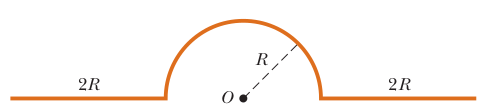
\includegraphics[scale=0.35]{./img/p1.png}
			\caption{Alambre cargado.}
			\label{p1}
		\end{figure}
	\end{ejercicio}
\end{mdframed}



\begin{mdframed}[style=warning]
	\begin{ejercicio}
		\textbf{Extra:} Resolver el problema $23.91$ de Zemansky 13ed. Vol. 2.
	\end{ejercicio}
\end{mdframed}





















































%%%